%%%%%%%%%%%%%%%%%%%%%%%%%%%%%%%%%%%%%%%%%
% Beamer Presentation
% LaTeX Template
% Version 1.0 (10/11/12)
%
% This template has been downloaded from:
% http://www.LaTeXTemplates.com
%
% License:
% CC BY-NC-SA 3.0 (http://creativecommons.org/licenses/by-nc-sa/3.0/)
%
%%%%%%%%%%%%%%%%%%%%%%%%%%%%%%%%%%%%%%%%%

%----------------------------------------------------------------------------------------
%	PACKAGES AND THEMES
%----------------------------------------------------------------------------------------

\documentclass{beamer}

\mode<presentation> {

% The Beamer class comes with a number of default slide themes
% which change the colors and layouts of slides. Below this is a list
% of all the themes, uncomment each in turn to see what they look like.

%\usetheme{default}
%\usetheme{AnnArbor}
%\usetheme{Antibes}
%\usetheme{Bergen}
%\usetheme{Berkeley}
%\usetheme{Berlin}
%\usetheme{Boadilla}
%\usetheme{CambridgeUS}
%\usetheme{Copenhagen}
%\usetheme{Darmstadt}
%\usetheme{Dresden}
\usetheme{Frankfurt}
%\usetheme{Goettingen}
%\usetheme{Hannover}
%\usetheme{Ilmenau}
%\usetheme{JuanLesPins}
%\usetheme{Luebeck}
%\usetheme{Madrid}
%\usetheme{Malmoe}
%\usetheme{Marburg}
%\usetheme{Montpellier}
%\usetheme{PaloAlto}
%\usetheme{Pittsburgh}
%\usetheme{Rochester}
%\usetheme{Singapore}
%\usetheme{Szeged}
%\usetheme{Warsaw}

% As well as themes, the Beamer class has a number of color themes
% for any slide theme. Uncomment each of these in turn to see how it
% changes the colors of your current slide theme.

%\usecolortheme{albatross}
%\usecolortheme{beaver}
%\usecolortheme{beetle}
%\usecolortheme{crane}
%\usecolortheme{dolphin}
%\usecolortheme{dove}
%\usecolortheme{fly}
%\usecolortheme{lily}
%\usecolortheme{orchid}
%\usecolortheme{rose}
%\usecolortheme{seagull}
%\usecolortheme{seahorse}
%\usecolortheme{whale}
%\usecolortheme{wolverine}

%\setbeamertemplate{footline} % To remove the footer line in all slides uncomment this line
%\setbeamertemplate{footline}[page number] % To replace the footer line in all slides with a simple slide count uncomment this line

%\setbeamertemplate{navigation symbols}{} % To remove the navigation symbols from the bottom of all slides uncomment this line
}

\usepackage{graphicx} % Allows including images
\usepackage{booktabs} % Allows the use of \toprule, \midrule and \bottomrule in tables
\usepackage{hyperref}
%----------------------------------------------------------------------------------------
%	TITLE PAGE
%----------------------------------------------------------------------------------------

\title[Latex Intro TCE]{Introduction to \\ \LaTeX \\ for creating PPTs and Reports} % The short title appears at the bottom of every slide, the full title is only on the title page

\author{Vetrivel Chelian T} % Your name
\institute[TCE] % Your institution as it will appear on the bottom of every slide, may be shorthand to save space
{
Thiagarajar College of Engineering \& Technology, Madurai \\ % Your institution for the title page
\medskip
\textit{vetrivelchelian@student.tce.edu} % Your email address
}
\date{\today} % Date, can be changed to a custom date

\begin{document}

\begin{frame}
\titlepage % Print the title page as the first slide
\end{frame}

\begin{frame}
\frametitle{Overview} % Table of contents slide, comment this block out to remove it
\tableofcontents % Throughout your presentation, if you choose to use \section{} and \subsection{} commands, these will automatically be printed on this slide as an overview of your presentation
\end{frame}

%----------------------------------------------------------------------------------------
%	PRESENTATION SLIDES
%----------------------------------------------------------------------------------------

%------------------------------------------------
\section{Installation} % Sections can be created in order to organize your presentation into discrete blocks, all sections and subsections are automatically printed in the table of contents as an overview of the talk
%------------------------------------------------

\subsection{Introduction} % A subsection can be created just before a set of slides with a common theme to further break down your presentation into chunks

\begin{frame}
\frametitle{\LaTeX}
\begin{itemize}
\item WYSIWIG ("what you see is what you get") word processors are Microsoft Word, LibreOffice Writer and Apple Pages. 
\item In LaTeX,the writer simply puts plain text in a given template adds formating to the text similar to markup styles (like HTML)
\item Mainly used by people in STEM (Science, Technology, Engineering and Mathematics) as Microsoft Word tend to be pretty bad at formatting equations.
%\item 
\end{itemize}
\end{frame}

%------------------------------------------------
\begin{frame}
\frametitle{why \LaTeX }
\begin{itemize}
\item LaTeX is the mathematical typesetting standard in all technical disciplines and in many Journals.
\item LaTeX is free and looks beautiful.
\item Start very small or use prebuilt templates and progress slowly
\item \url{https://tex.stackexchange.com/} use this site whenever needed
\item learn as you progress, for a first few times might be counter intuitive but as you get used to LateX it will save us lots of time
\end{itemize}
\end{frame}
%--------------------------------------------------
\begin{frame}
\frametitle{why \LaTeX }
\begin{itemize}
\Large \item Table of contents is automatically generated including page number
\item List of figures and List of tables automatically generated
\item References are automatically generated
\item Text is always formatted and clean with what you have given in header
\item Images numberings,Tables numberings and Equation numberings are automatic and are beautiful to look at
\end{itemize}
\end{frame}
%------------------------------------------------
\begin{frame}
\frametitle{LaTeX vs Word}
%
\begin{center}
%
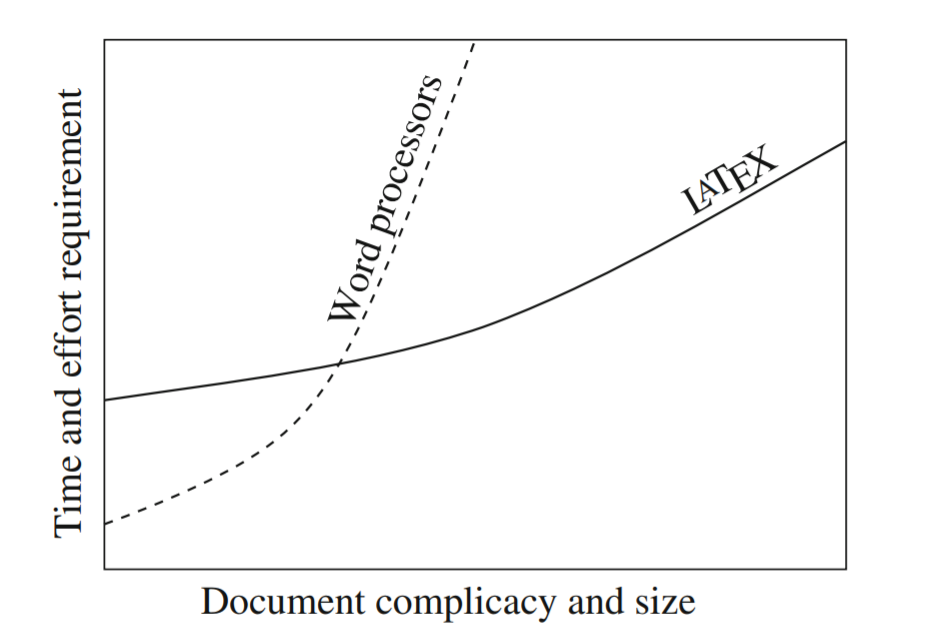
\includegraphics[width=0.75\linewidth]{complexity}
\end{center}
%
\end{frame}
%--------------------------------------------
\begin{frame}
\frametitle{LaTeX vs Word}
%
\begin{center}
%

\includegraphics[width=0.75\linewidth]{144}
\end{center}
%
Latex decides where to put figures and tables for best fit automatically.
\end{frame}
\subsection{Installation} 

%--------------------------------------------
\begin{frame}
\frametitle{Backend and Frontend}
\begin{itemize}
\item First we need to install MiKTeX backend for LaTeX.
\item I prefer using TexWorks(Frontend) as its simple to use and faster to deploy.
\item One can explore other IDEs for TeX formatting.
\item MiKTeX can be downloaded from \url{https://miktex.org/download}.
\item Installation Guide from \url{https://miktex.org/howto/install-miktex}.
%\item Nam cursus est eget velit posuere pellentesque
%\item Vestibulum faucibus velit a augue condimentum quis convallis nulla gravida
\end{itemize}

\end{frame}

%------------------------------------------------

\begin{frame}
\frametitle{Creating Documents and Presentations}
\begin{block}{For creating PPTs}
Just initialise document class as  beamer
\end{block}

\begin{block}{For Creating Documents}

Just initialise document class as a4paper and article

\end{block}

\begin{block}{Using Prebuilt Templates}
Search google for templates and start using them directly (easiest method)
\end{block}
\end{frame}

%------------------------------------------------

\begin{frame}
\frametitle{Multiple Columns}
\begin{columns}[c] % The "c" option specifies centered vertical alignment while the "t" option is used for top vertical alignment

\column{.45\textwidth} % Left column and width
\textbf{Heading}
\begin{enumerate}
\item Statement
\item Explanation
\item Example
\end{enumerate}

\column{.5\textwidth} % Right column and width
Lorem ipsum dolor sit amet, consectetur adipiscing elit. Integer lectus nisl, ultricies in feugiat rutrum, porttitor sit amet augue. Aliquam ut tortor mauris. Sed volutpat ante purus, quis accumsan dolor.

\end{columns}
\end{frame}

%------------------------------------------------
\section{Using LaTeX}
%------------------------------------------------

\begin{frame}
\frametitle{Table}
\begin{table}
\begin{tabular}{l l l}
\toprule
\textbf{Treatments} & \textbf{Response 1} & \textbf{Response 2}\\
\midrule
Treatment 1 & 0.0003262 & 0.562 \\
Treatment 2 & 0.0015681 & 0.910 \\
Treatment 3 & 0.0009271 & 0.296 \\
\bottomrule
\end{tabular}
\caption{Table caption}
\end{table}
\end{frame}

%------------------------------------------------

\begin{frame}
\frametitle{Theorem}
\begin{theorem}[Mass--energy equivalence]
$E = mc^2$
\end{theorem}
\end{frame}

%------------------------------------------------
\subsection{Simple Document Creation}
\begin{frame}[fragile] % Need to use the fragile option when verbatim is used in the slide
\frametitle{First Latex Document}

\begin{verbatim}

\documentclass[a4paper,12pt]{report}
\usepackage[left=35mm, right=25mm, top=25mm]{geometry}
\usepackage{setspace}
\linespread{1.5}
\usepackage{times}
\begin{document}
.
.
.
\end{document}
\end{verbatim}
\end{frame}
%------------------------------------------------

\subsection{Inserting Image}
\begin{frame}[fragile]
\frametitle{Figure}
\begin{verbatim}
\usepackage{graphicx}%must be included in header
\begin{figure}
\includegraphics[width=0.8\linewidth]{test}
%image should in same folder as .tex files
\end{figure}
\end{verbatim}
\end{frame}

%------------------------------------------------

\begin{frame}[fragile] % Need to use the fragile option when verbatim is used in the slide
\frametitle{Citation}
An example of the \verb|\cite| command to cite within the presentation:\\~

This statement requires citation \cite{p1}.
\end{frame}

%------------------------------------------------

\begin{frame}
\frametitle{References}
\footnotesize{
\begin{thebibliography}{99} % Beamer does not support BibTeX so references must be inserted manually as below
\bibitem[Smith, 2012]{p1} John Smith (2012)
\newblock Title of the publication
\newblock \emph{Journal Name} 12(3), 45 -- 678.
\end{thebibliography}
}
\end{frame}

%------------------------------------------------

\begin{frame}
\Huge{\centerline{The End}}
\end{frame}

%----------------------------------------------------------------------------------------

\end{document} 